\documentclass[a4paper,11pt]{article}

%--------------------------------------------------------------------
% PACKAGES
%--------------------------------------------------------------------
\usepackage{fontspec}
\usepackage[greek,english]{babel} % Greek + English
\usepackage{xcolor}
\usepackage{xgreek}               % For Greek text
\usepackage{tcolorbox}
\usepackage{hyperref}
\usepackage{enumitem}
\usepackage{graphicx}             % For including images
\usepackage{float}                % For positioning images with 'H' option
\usepackage{caption}
\usepackage{subcaption}
\usepackage{listings}
\usepackage{fmtcount}
\usepackage{titlesec}
\usepackage{minted}
\usepackage{float}
\usepackage{subcaption}
\usepackage[a4paper, margin=1in]{geometry}
\usepackage{titlesec}


%--------------------------------------------------------------------
% FONTS & LAYOUT ADJUSTMENTS (optional)
%--------------------------------------------------------------------
% If you face issues with Greek in fontspec-based LaTeX compilers (XeLaTeX/LuaLaTeX),
% set a main font that supports Greek.
%\setmainfont{Times New Roman} % or any other that has Greek glyphs
\usemintedstyle{friendly}
\setmainfont{Times New Roman}

\lstdefinelanguage{json}{
  basicstyle=\ttfamily\small,
  commentstyle=\color{green!50!black},
  stringstyle=\color{red!50!black},
  showstringspaces=false,
  breaklines=true,
  % possibly more rules for keywords, etc.
}

\titlespacing*{\section}
  {0pt}    % left indentation
  {4em}    % space before (vertical)
  {1em}    % space after (vertical)
\titlespacing*{\subsection}
  {0pt}
  {4em}
  {0.5em}



%--------------------------------------------------------------------
% DOCUMENT
%--------------------------------------------------------------------
\begin{document}
\selectlanguage{greek}

\title{\textbf{Αναφορά: Πρόβλεψη Alzheimer’s με Χρήση Νευρωνικών Δικτύων}}
\author{\\
\large Νίκος Ανδριανόπουλος \\
\large Α.Μ. φοιτητή: 1084637 \\
\large \texttt{up1084637@ac.upatras.gr}
}
\date{\today}
\maketitle

\tableofcontents
%--------------------------------------------------------------------
% 1. ΕΙΣΑΓΩΓΗ
%--------------------------------------------------------------------
\section{Εισαγωγή}
Στην παρούσα εργασία μελετάω τη χρήση Τεχνητών Νευρωνικών Δικτύων (ΤΝΔ) για την
πρόβλεψη της νόσου Alzheimer, χρησιμοποιώντας το σύνολο δεδομένων που παρέχεται
(Alzheimer’s Disease Dataset). Στόχος είναι να ταξινομήσουμε ασθενείς σε δύο κλάσεις
(Alzheimer ή μη) βάσει διαφόρων χαρακτηριστικών (βιοδείκτες, συμπτώματα, κ.λπ.).

Παρακάτω παρουσιάζονται τα βήματα που ακολουθήθηκαν, σύμφωνα με τα ερωτήματα του
Μέρους Α’ της εργασίας.Τα αποτελέσματα είναι κομμάτια των json αρχείων που δημιουργούνται μετά
την εκτέλεση του κώδικα, βάζω την χρήσιμη πληροφορία για την απάντηση του κάθε ερωτήματος όχι όλο το json.
Οι τιμές μπορεί να είναι λιγο διαφορετικές, επειδή χρησιμοποιείται η gpu από ερώτημα σε ερώτημα αλλά οι διαφορές 
μεταξύ των τιμών είναι πάντα σταθερές(π.χ.η=0.001 δίνει καλύτερη απόδοση απο η=0.05).
%--------------------------------------------------------------------
% A1. ΠΡΟΕΠΕΞΕΡΓΑΣΙΑ
%--------------------------------------------------------------------
\section{A1: Προεπεξεργασία και Προετοιμασία Δεδομένων}

\subsection{(α) Κωδικοποίηση και προεπεξεργασία δεδομένων}
Στο σύνολο δεδομένων εντοπίστηκαν κατηγορικές και ποσοτικές μεταβλητές, οπότε:
\begin{itemize}
    \item \textbf{One-hot encoding:} Εφαρμόστηκε στις κατηγορικές στήλες:\emph{Εthnicity}, \emph{Education Level}, οι οποίες έχουν τιμές στο [0,3].Πρέπει να γίνει αυτή η αλλαγή καθώς το 0 από το 3 στη
    συγκεκριμένη περίπτωση δεν έχει κάποια επιπλέον πληροφορία αλλά αν το αθροίσουμε επειδή είναι μεγαλύτερος αριθμός θα δώσει.
    \item \textbf{Κανονικοποίησής/Τυποποίηση:} (Π.χ.) Χρησιμοποιήθηκε η \emph{z-score} μέθοδος για να παρέχω στις στήλες με συνεχείς τιμές στατιστικές ιδιότητες.
    \item Για τις στήλες που έχουν δυαδικές τιμές δεν κάνω κάποια αλλαγή γιατί δεν υπάρχει κίνδυνος υπερεκτίμησης της πληροφορίας.
    % ή
    % Χρησιμοποιήθηκε η τυποποίηση (z-score) ώστε κάθε χαρακτηριστικό να έχει μέση τιμή 0 και τυπική απόκλιση 1.
\end{itemize}

Στις συνεχείς στήλες βέβαια μπορώ να κάνω  centering και min-max, αλλά η τυποποίηση είναι καλύτερη και από τις 2 μεθόδους γιατί κεντράρει αλλά και κλιμακώνει ταυτόχρονα 
τα δεδομένα, όλα τα χαρακτηριστικά συνεισφέρουν ομοιόμορφα στη μάθηση.Στην πράξη:

\begin{minted}[breaklines, fontsize=\small]{json}
    {
        "pre_processing":"centering"
        "Average loss": 0.5412922739982605,
        "Average Accuracy": 0.7603491067886352,
        "Average MSE": 0.16807735860347747
    }
    \end{minted}

\begin{minted}[breaklines, fontsize=\small]{json}
    {
        "pre_processing":"min-max"
        "Average loss": 0.3923275530338287,
        "Average Accuracy": 0.8306109428405761,
        "Average MSE": 0.1211971566081047
    }
    \end{minted}

\begin{minted}[breaklines, fontsize=\small]{json}
    {
        "pre_processing":"z-score"    
        "Average loss": 0.39323789477348325,
        "Average Accuracy": 0.8394557356834411,
        "Average MSE": 0.12149734944105148
    }
    \end{minted}

\newpage
\noindent
\textbf{Κώδικας του pre-processing}:
\begin{minted}[frame=single, linenos]{python}
    def min_max(panda,columns):
        scaler = MinMaxScaler(feature_range=(-1, 1))
        normalized_data = scaler.fit_transform(panda[columns])

        return normalized_data

    def centering(panda,columns):
        scaler = StandardScaler(with_std=False)  
        centered_data = scaler.fit_transform(panda[columns])

        return centered_data

    def z_score(panda,columns):
        scaler = StandardScaler()  
        cont_val=panda[columns]
        zscored_data = scaler.fit_transform(panda[columns])

        return zscored_data
    \end{minted}
    

Τέλος κάνω concatenate τα δεδομένα μώλις γίνουν numpy arrays και τα κάνω cast όλα σε float32, επειδή 
βοηθάει τις gpu στις πράξεις.

\begin{minted}[frame=single, linenos]{python}
filtered_input=np.concatenate([pre_processed_input, \
encoded_input,binary_input], axis=1).astype(np.float32)
    \end{minted}

    \begin{figure}[H]
      \centering
      \begin{subfigure}{0.70\textwidth}
        \includegraphics[width=\linewidth]{screenshots/SGD_mom0.0_lr0.001_two_thirds_Relu_cross entropy_None_more_layers_04_06_11_01_58/Plot.png}
        \caption{Centering}
        \label{fig:sub1}
      \end{subfigure}
      \quad
      \begin{subfigure}{0.70\textwidth}
        \includegraphics[width=\linewidth]{screenshots/SGD_mom0.0_lr0.001_two_thirds_Relu_cross entropy_None_more_layers_04_06_11_06_53/Plot.png}
        \caption{Min-max}
        \label{fig:sub2}
      \end{subfigure}
      \begin{subfigure}{0.70\textwidth}
        \includegraphics[width=\linewidth]{screenshots/SGD_mom0.0_lr0.001_two_thirds_Relu_cross entropy_None_more_layers_04_06_11_11_44/Plot.png}
        \caption{z-score}
        \label{fig:sub2}
      \end{subfigure}
      \caption{Όπως φαίνεται από τις γραφικές παραστάσεις και τα αποτελέσματα το z-score έχει καλύτερη απόδοση, μικρό loss και πιο ομαλές γραφικές παραστάσεις.}
      \label{fig:two_plots}
    \end{figure}
    


    

\subsection{(β) Διασταυρούμενη Επικύρωση (5-fold CV)}
Για την αξιόπιστη εκτίμηση των επιδόσεων των μοντέλων, χρησιμοποιήθηκε \emph{5-fold
Cross Validation}.Τα folds να είναι \emph{ισορροπημένα} ως προς
τον αριθμό δειγμάτων ανά κλάση. Σε κάθε πείραμα:
\begin{itemize}
    \item Διαχωρίστηκαν τα δεδομένα σε 5 $\approx$ ίσα τμήματα (folds).
    \item Κάθε φορά, 4 folds χρησιμοποιήθηκαν για εκπαίδευση και 1 για έλεγχο.
    \item Επαναλήφθηκε η διαδικασία 5 φορές και υπολογίστηκε ο μέσος όρος των μετρικών.
\end{itemize}

\textbf{Κώδικας του pre-processing}:
\begin{minted}[frame=single, linenos, fontsize=\footnotesize]{python}
def normal_training(filtered_input,output,args,folder,hidden_layers):
        five_fold = StratifiedKFold(n_splits=5, shuffle=True, random_state=44) 
        round=1
        evals=[]
        val_loss_table=[]
        loss_table=[]
        early_stop_epochs=[]
        batch_size=32

        for training_idx,val_idx in five_fold.split(filtered_input,output):

            input_train,input_val=filtered_input[training_idx],filtered_input[val_idx]
            output_train,output_val=output[training_idx],output[val_idx]

            
            model,early_stop=nn_model(parameters)
            training=model.fit(input_train, output_train,
            validation_data=(input_val, output_val),epochs=args.epochs, batch_size=batch_size)

            stop_epoch=len(training.history['loss'])
            early_stop_epochs.append(stop_epoch)

            val_loss_table.append(training.history['val_loss'])
            loss_table.append(training.history['loss'])
    \end{minted}

\begin{minted}[frame=single, linenos, fontsize=\footnotesize]{python}
    parameters:
    filtered_input.shape[1],
    args.optimizer,
    args.momentum,
    args.lr,
    args.num_of_layers,
    args.hid_layer_func,
    args.loss_func,
    args.use_l2,
    args.use_l1,
    args.r,
    args.more_layers,
    hidden_layers
    \end{minted}

Οι παραμέτροι κυρίως είναι για τα επόμενα ερωτήματα και εξηγούνται πλήρως στον parser του κώδικα στο github, ορισμένοι 
θα εξηγηθούν στα επόμενα ερωτήματα.

\begin{figure}[H]
    \centering
    \includegraphics[width=0.7\textwidth]{/home/nikolis/Desktop/5o_etos/ai/predicting_alzheimers/latex/screenshots/pr.png}
    \caption{Το split έχει γίνει σωστά και ισορροπημένα}
    \label{fig:two_thirds}
\end{figure}
%--------------------------------------------------------------------
% A2. ΕΠΙΛΟΓΗ ΑΡΧΙΤΕΚΤΟΝΙΚΗΣ
%--------------------------------------------------------------------
\section{A2: Επιλογή Αρχιτεκτονικής}

\subsection{(α) Σημασία των μετρικών CE, MSE, Accuracy}
\begin{itemize}
  \item \textbf{Cross-Entropy (CE) loss:} Καταλληλότερη σε περιπτώσεις ταξινόμησης, καθώς τιμωρεί έντονα σφάλματα στην πιθανότητα της σωστής κλάσης και συνήθως οδηγεί σε καλύτερη σύγκλιση.
  \item \textbf{Μέσο Τετραγωνικό Σφάλμα (MSE):} Χρησιμοποιείται συχνά σε προβλήματα παλινδρόμησης. Σε ταξινόμηση μπορεί να οδηγήσει σε βραδύτερη/όχι ιδανική σύγκλιση.Εδώ χρησιμοποιείται μόνο σαν μέτρο της 
  απόστασης των προβλέψεων από τις validation τιμές, για τη σύγκριση των διαφόρων πειραμάτων.
  \item \textbf{Ακρίβεια (Accuracy):} Αφορά το ποσοστό σωστών προβλέψεων. Δεν είναι συνήθως η βέλτιστη \emph{συνάρτηση κόστους} για εκπαίδευση.Τη χρησιμοποιώ πάλι για τη σύγκριση των πειραμάτων.
\end{itemize}
\noindent
\textbf{Συμπέρασμα:} Για την εκπαίδευση (loss) χρησιμοποιώ CE, ενώ για αναφορά
τελικών επιδόσεων χρησιμοποιώ ακρίβεια.Προεραιτικά χρησιμοποιώ και MSE μαζί με την ακρίβεια για τη σύγκριση των επιδόσεων.

\subsection{(β) Αριθμός νευρώνων στο επίπεδο εξόδου}
Για μια \emph{binary classification} (Alzheimer ή μη) αρκεί:
\begin{itemize}
    \item 1 νευρώνας εξόδου με σιγμοειδή λειτουργία (παραγωγή $x \in (0,1)$), ή
    \item 2 νευρώνες εξόδου με \emph{Softmax}, με one hot encoding (πιο γενικευμένη προσέγγιση).
\end{itemize}
Και τα 2 βγάζουν ίδια αποτελέσματα, οποτέ υλοποιώ το πιο απλό(Sigmoid):
\begin{minted}[breaklines, fontsize=\small]{json}
    {
        "softax":"yes",
        "Average loss": 0.39862353801727296,
        "Average Accuracy": 0.8397802214622497,
        "Average MSE": 0.12448595911264419

        ========================================
        
        "sigmoid":"yes",
        "Average loss":0.39606810808181764
        "Average Accuracy":0.83433837890625
        "Average MSE":0.1230233833193779

      }
    \end{minted}

\subsection{(γ) Επιλογή συνάρτησης ενεργοποίησης στους κρυφούς κόμβους}
\begin{itemize}
    \item \textbf{Tanh:} Καλύτερη κλίμακα τιμών από τη σιγμοειδή (παράγει τιμές σε $[-1, 1]$), αλλά μπορεί να υποφέρει από vanishing gradients.
    \item \textbf{ReLU:} Συχνά προτιμάται σε βαθιά δίκτυα, έχει γρήγορη σύγκλιση, αλλά υπάρχει η περίπτωση “dying ReLUs”.
    \item \textbf{SiLU:} Εναλλακτική που σε ορισμένες περιπτώσεις ξεπερνά σε επίδοση το ReLU, αλλά είναι πιο σύνθετη.
\end{itemize}
\noindent
Πάλι όλες βγάζουν παρόμοια αποτελέσματα οπότε επιλέγω την πιο απλή και πιο ευρέως προτιμημένη:
\begin{minted}[breaklines, fontsize=\small]{json}
    {
        "hidden layer activation function":"Tanh",
        "Average loss": 0.39862353801727296,
        "Average Accuracy": 0.8334038019180298,
        "Average MSE": 0.11632926613092423

        ========================================
        
        "hidden layer activation function":"Silu",
        "Average loss":0.39606810808181764
        "Average Accuracy":0.83433837890625
        "Average MSE":0.1230233833193779

        ========================================

        "hidden layer activation function":"Relu"    
        "Average loss": 0.39323789477348325,
        "Average Accuracy": 0.8394557356834411,
        "Average MSE": 0.12149734944105148

      }
    \end{minted}


\subsection{(δ) Συνάρτηση ενεργοποίησης στο επίπεδο εξόδου}
\begin{itemize}
    \item Εξηγήθηκε πριν, έχει επιλεχτεί η Sigmoid.
\end{itemize}
\newpage
\subsection{(ε) Αριθμός νευρώνων στο κρυφό επίπεδο και αποτελέσματα}
 $I$=38 είναι ο αριθμός εισόδων. Aκολουθούν τιμές και γραφήματα σύγκλισης:

\begin{center}
\begin{tabular}{|c|c|c|c|}
\hline
\textbf{Νευρώνες $H$} & \textbf{CE Loss} & \textbf{MSE} & \textbf{Accuracy} \\
\hline
$I/2$   & 0.3937569260597229 & 0.12326516360044479 &0.8310836553573608  \\
\hline
$2I/3$  & 0.3960006356239319 & 0.12397604882717132 & 0.8320052027702332 \\
\hline
$I$     & 0.3982479512691498 & 0.12300745993852616& 0.8310847401618957 \\
\hline
$2I$    & 0.3929096460342407 & 0.12164172381162644  & 0.8329386830329895\\
\hline
\end{tabular}
\end{center}

\begin{figure}[H]
    \centering
    \includegraphics[width=0.7\textwidth]{/home/nikolis/Desktop/5o_etos/ai/predicting_alzheimers/latex/screenshots/Figure_1.png}
    \caption{Οι τιμές σε γράφημα}
    \label{fig:double}
\end{figure}


\begin{figure}[H]
    \centering
    \includegraphics[width=0.7\textwidth]{/home/nikolis/Desktop/5o_etos/ai/predicting_alzheimers/screenshots/SGD_mom0.0_lr0.001_double_Relu_cross entropy_None_04-03_21-34-38/Plot.png}
    \caption{2*I}
    \label{fig:double}
\end{figure}

\begin{figure}[H]
    \centering
    \includegraphics[width=0.7\textwidth]{/home/nikolis/Desktop/5o_etos/ai/predicting_alzheimers/screenshots/SGD_mom0.0_lr0.001_half_Relu_cross entropy_None_04-03_21-42-33/Plot.png}
    \caption{I/2}
    \label{fig:half}
\end{figure}

\begin{figure}[H]
    \centering
    \includegraphics[width=0.7\textwidth]{/home/nikolis/Desktop/5o_etos/ai/predicting_alzheimers/screenshots/SGD_mom0.0_lr0.001_same_Relu_cross entropy_None_04-03_21-30-46/Plot.png}
    \caption{I}
    \label{fig:same}
\end{figure}

\begin{figure}[H]
    \centering
    \includegraphics[width=0.7\textwidth]{screenshots/SGD_mom0.0_lr0.001_two_thirds_Relu_cross entropy_None_more_layers_04_06_11_11_44/Plot.png}
    \caption{2*I/3}
    \label{fig:two_thirds}
\end{figure}


\noindent
\textbf{Συμπεράσματα:}
\begin{itemize}
    \item \emph{(i)} Κατάλληλος αριθμός κρυφών νευρώνων: 2*I, Όπως φαίνεται και από πάνω τα καλύτερα αποτελέσματα τα δίνει ο μεγαλύτερος αριθμός νευρώνων.
    Επιπλέον, εκτός από το καλύτερο accuracy έχει το την πιο χαμηλή και ομαλή συνάρτηση validation loss:

    \begin{figure}[H]  % or [htbp]
        \centering
        \includegraphics[width=1\textwidth]{screenshots/1.png}
        \caption{Validation-loss plot για τα διαφορετικά νούμερα νευρώνων}
        \label{fig:acc_vs_epochs}
      \end{figure}
      

    \item \emph{(ii)} Συνάρτηση κόστους που δίνει βέλτιστη απόδοση: Binary-Crossentropy, το πρόβλημα είναι δυαδική ταξινόμηση οπότε, η συνάρτηση που 
    μετράει πόσο διαφέρει η πρόβλεψη από την πραγματική τιμή για ένα δυαδικό αποτέλεσμα είναι η φυσική επιλογή. 
    \item \emph{(iii)} Συνάρτηση ενεργοποίησης που οδηγεί σε βέλτιστη μάθηση: Relu όπως εξηγήθηκε.
    \item \emph{(iv)} Ταχύτητα σύγκλισης / εποχές εκπαίδευσης: Για να βρώ τα κατάλληλα epochs που αρχίζει να υπερεκπεδεύται το δείγμα, αρκεί να κάνω το plot Training-Validation loss και να δω
    από ποιο epoch αρχίζει το validation-loss να παραμένει σταθερό ενώ το training συνεχίζει να μειώνεται:

    \begin{figure}[H]
        \centering
        \includegraphics[width=0.7\textwidth]{screenshots/2.png}
        \caption{Περίπου στα 600 epochs συμβαίνει το φαινόμενο.}
        \label{fig:two_thirds}
    \end{figure}
\end{itemize}

\subsection{(στ) Κριτήριο τερματισμού}
Χρησιμοποιήθηκε  \emph{early stopping}:
\begin{itemize}
    \item Παρακολουθώ το validation loss στο validation fold.
    \item Αν για 10 συνεχόμενες εποχές δεν βελτιώνεται κατά μια σταθερά(0.001) η CE, το σταματάω.
\end{itemize}

Με early stopping επιβεβαιώνεται και η παρατήρηση για τη σύγκλισή των epochs:

\begin{figure}[H]  % or [htbp]
    \centering
    \includegraphics[width=1\textwidth]{/home/nikolis/Desktop/5o_etos/ai/predicting_alzheimers/latex/screenshots/SGD_mom0.0_lr0.001_two_thirds_Relu_cross entropy_None_more_layers_04-06_16-51-07/Plot.png}
    \caption{Εarly stopping κοντά στα 600 epochs}
    \label{fig:acc_vs_epochs}
  \end{figure}

\newpage
\textbf{Κώδικας:}
\begin{minted}[frame=single, linenos]{python}
    early_stopping = tf.keras.callbacks.EarlyStopping(
        monitor='val_loss', 
        patience=10,
        min_delta=0.001,              
        restore_best_weights=True  
    )
    \end{minted}

%--------------------------------------------------------------------
% A3. ΜΕΤΑΒΟΛΕΣ ΣΕ ΡΥΘΜΟ ΕΚΠΑΙΔΕΥΣΗΣ (η) ΚΑΙ ΣΤΑΘΕΡΑ ΟΡΜΗΣ (m)
%--------------------------------------------------------------------
\section{A3: Μεταβολές στον ρυθμό εκπαίδευσης και στη σταθερά ορμής}
Έπειτα από επιλογή της καλύτερης τοπολογίας στο Α2, πειραματιστήκαμε με διαφορετικές
τιμές $\eta$ και $m$ (learning rate και momentum). Ο πίνακας συνοψίζει τα αποτελέσματα
μετά από 5-fold CV:

\begin{center}
\begin{tabular}{|c|c|c|c|c|}
\hline
\textbf{$\eta$} & \textbf{$m$} & \textbf{CE Loss} & \textbf{MSE} & \textbf{Accuracy} \\
\hline
0.001 & 0.2 & 0.3862103223800659 & 0.11963917911052704 & 0.8366617918014526 \\
\hline
0.001 & 0.6 & 0.37646722197532656 & 0.11473272740840912 & 0.8413118839263916 \\
\hline
0.05  & 0.6 & 0.3590724289417267 & 0.1064189225435257 & 0.8599360227584839 \\
\hline
0.1   & 0.6 & 0.36190045475959776 & 0.10914652198553085 & 0.8464411616325378 \\
\hline
\end{tabular}
\end{center}

\begin{figure}[H]
    \centering
    \includegraphics[width=0.7\textwidth]{/home/nikolis/Desktop/5o_etos/ai/predicting_alzheimers/latex/screenshots/Figure_2.png}
    \caption{Οι τιμές σε γράφημα}
    \label{fig:double}
\end{figure}

\begin{figure}[H]
    \centering
    \includegraphics[width=0.7\textwidth]{/home/nikolis/Desktop/5o_etos/ai/predicting_alzheimers/screenshots/SGD_mom0.2_lr0.001_double_Relu_cross entropy_None_04-03_21-46-38/Plot.png}
    \caption{m=0.2,η=0.001}
    \label{fig:double}
\end{figure}

\begin{figure}[H]
    \centering
    \includegraphics[width=0.7\textwidth]{/home/nikolis/Desktop/5o_etos/ai/predicting_alzheimers/screenshots/SGD_mom0.6_lr0.001_double_Relu_cross entropy_None_04-03_21-50-11/Plot.png}
    \caption{m=0.6,η=0.001}
    \label{fig:half}
\end{figure}

\begin{figure}[H]
    \centering
    \includegraphics[width=0.7\textwidth]{/home/nikolis/Desktop/5o_etos/ai/predicting_alzheimers/latex/screenshots/SGD_mom0.6_lr0.05_double_Relu_cross entropy_None_more_layers_04-06_17-04-49/Plot.png}
    \caption{m=0.6,η=0.05}
    \label{fig:same}
\end{figure}

\begin{figure}[H]
    \centering
    \includegraphics[width=0.7\textwidth]{/home/nikolis/Desktop/5o_etos/ai/predicting_alzheimers/screenshots/SGD_mom0.6_lr0.1_double_Relu_cross entropy_None_04-03_21-52-53/Plot.png}
    \caption{m=0.6,η=0.01}
    \label{fig:two_thirds}
\end{figure}

\noindent
\textbf{Γιατί $m < 1$:} To momentum καθορίζει πόσο μέρος της ενημέρωσης των βαρών απο την προηγούμενη χρονική στιγμή συνυπολογίζεται με το τωρινό:
\(\Delta w_{t} = m\,\Delta w_{t-1} \;-\; \eta\,\nabla J\bigl(w_{t-1}\bigr)\).
Οπότε άν το m>1 μετά από πολλούς κύκλους ο όρος \( m\,\Delta w_{t-1} \) θα γινόταν τεράστιος ,δυσκολεύοντας έτσι την σύγκλιση λόγω τεράστιων βημάτων και θα εγκλωβιζόταν σε τοπικά ελάχιστα.


\noindent
\textbf{Συμπεράσματα:} Αν και για m=0.6,η=0.05 φαίνεται πως έχει τα καλύτερα αποτελέσματα, από τις γραφικές παραστάσεις φαίνεται πως η εκπαίδευση δεν είναι ομαλή και υπάρχει overfitting και σταδιακή αύξηση του loss.
Γι αυτό επιλέγεται το m=0.6,η=0.001 που συγκλίνει στα μισά epochs από m=0/0.2 είναι ομαλό και έχει πολυ καλές μέσες τιμές.\\Όπως φαίνεται από τις 2 τελευταίες γραφικές παραστάσεις όσο αυξάνεις το η τόσο πιο απότομες κινήσεις γίνονται με σκοπό την εύρεση του ελαχίστου, 
πράγμα που μπορεί να εγκλωβίζει την εκπαίδευση σε τοπικά ελάχιστα.Ο συνδυασμός κατάλληλου m  ώστε μαζί με σχετικά μικρό η, δίνει το κατάλληλο άλμα(καθώς το m βασίζεται στις προηγούμενες θέσεις) και μειώνει τον αριθμό των epochs.

%--------------------------------------------------------------------
% A4. ΚΑΝΟΝΙΚΟΠΟΙΗΣΗ (REGULARIZATION)
%--------------------------------------------------------------------
\newpage
\section{A4: Ομαλοποίηση (Regularization)}
Για την αποφυγή υπερπροσαρμογής (overfitting), δοκιμάζω L1 και L2.Κάνω εκπαίδευση για 600 epochs.


\begin{center}
\begin{tabular}{|c|c|c|c|}
\hline
\textbf{$L1(r)$} & \textbf{CE Loss} & \textbf{Accuracy} & \textbf{MSE} \\
\hline
0.0001 & 0.4038295090198517 & 0.8445785284042359 & 0.11286317259073257 \\
\hline
0.001  & 0.5127061903476715 & 0.8585396051406861 & 0.10416208952665329 \\
\hline
0.01   & 0.43445379137992857 & 0.8566726207733154 & 0.11263947784900666 \\
\hline
\end{tabular}
\end{center}

\begin{figure}[H]
    \centering
    \includegraphics[width=0.7\textwidth]{/home/nikolis/Desktop/5o_etos/ai/predicting_alzheimers/screenshots/SGD_mom0.6_lr0.001_double_Relu_cross entropy_0.0001_04_03_21_53_08/Plot.png}
    \caption{r=0.0001}
    \label{fig:double}
\end{figure}

\begin{figure}[H]
    \centering
    \includegraphics[width=0.7\textwidth]{/home/nikolis/Desktop/5o_etos/ai/predicting_alzheimers/screenshots/SGD_mom0.6_lr0.001_double_Relu_cross entropy_0.001_04_03_21_55_20/Plot.png}
    \caption{r=0.001}
    \label{fig:half}
\end{figure}

\begin{figure}[H]
    \centering
    \includegraphics[width=0.7\textwidth]{/home/nikolis/Desktop/5o_etos/ai/predicting_alzheimers/screenshots/SGD_mom0.6_lr0.001_double_Relu_cross entropy_0.01_04_03_21_57_50/Plot.png}
    \caption{r=0.01}
    \label{fig:same}
\end{figure}

\vspace{4em}
\begin{center}
\begin{tabular}{|c|c|c|c|}
\hline
\textbf{$L2(r)$} & \textbf{CE Loss} & \textbf{Accuracy} & \textbf{MSE} \\
\hline
0.0001 & 0.3834355592727661 & 0.8389960289001465 & 0.11614608764648438 \\
\hline
0.001  & 0.4198959469795227 & 0.8348034858703614 & 0.11451027244329452 \\
\hline
0.01   & 0.4104568600654602 & 0.856679129600525 & 0.10613797605037689 \\
\hline
\end{tabular}
\end{center}

\begin{figure}[H]
    \centering
    \includegraphics[width=0.7\textwidth]{/home/nikolis/Desktop/5o_etos/ai/predicting_alzheimers/screenshots/SGD_mom0.6_lr0.001_double_Relu_cross entropy_0.0001_04_03_22_02_21/Plot.png}
    \caption{r=0.0001}
    \label{fig:double}
\end{figure}

\begin{figure}[H]
    \centering
    \includegraphics[width=0.7\textwidth]{/home/nikolis/Desktop/5o_etos/ai/predicting_alzheimers/screenshots/SGD_mom0.6_lr0.001_double_Relu_cross entropy_0.001_04-03_22_04_47/Plot.png}
    \caption{r=0.001}
    \label{fig:half}
\end{figure}

\begin{figure}[H]
    \centering
    \includegraphics[width=0.7\textwidth]{/home/nikolis/Desktop/5o_etos/ai/predicting_alzheimers/screenshots/SGD_mom0.6_lr0.001_double_Relu_cross entropy_0.01_04_03_22_09_17/Plot.png}
    \caption{r=0.01}
    \label{fig:same}
\end{figure}

\vspace{4em}

\textbf{Τρέχω τη καλύτερη τιμή του L1 για 1300 epochs }
\begin{center}
    \begin{tabular}{|c|c|c|c|}
    \hline
    \textbf{$L2(r)$} & \textbf{CE Loss} & \textbf{Accuracy} & \textbf{MSE} \\
    \hline
    0.0001 & 0.4378849983215332 & 0.8636569499969482 & 0.09974857568740844 \\
    \hline
    \end{tabular}
    \end{center}

    \begin{figure}[H]
        \centering
        \includegraphics[width=0.7\textwidth]{/home/nikolis/Desktop/5o_etos/ai/predicting_alzheimers/screenshots/last/Plot.png}
        \caption{Θέλει πάνω απο 1000 epochs για σύγκλιση}
        \label{fig:same}
    \end{figure}

\noindent
\textbf{Συμπεράσματα:} Τα καλύτερα accuracies τα δίνει το L1 και φαίνεται πως χρειάζεται παραπάνω από 600 epochs όπως επιλέχθηκαν πριν για να συγκλίνει 
ιδιαίτερα για το r=0.001 που δίνει την μεγαλύτερη ακρίβεια.Το L2 ωστόσο δεν χάνει υπερβολικά στην ακρίβεια σε σχέση με το L1 και συγκλίνει πιο γρήγορα.\\
Τέλος, το L2 για να έχει την καλύτερη απόδοση πρέπει έχει μεγάλο r σε αντίθεση με το L1 που χάνει ακρίβεια.\\
Τα αποτελέσματα βγάζουν νόημά και για τις 2 περιπτώσεις.Το L1 εξαφανίζει τα άχρηστα χαρακτηριστικά μηδενίζοντας τα βάρη τους, οπότε σε 1 μικρό Dataset
όπως αυτό βγάζει καλύτερα αποτελέσματα.Το L2 ρυθμίζει πιο ομαλά τα βάρη  και ίσως σε περισσότερα δεδομένα θα ήταν καλύτερος εκτιμητής.Οπότε εν τέλει 
έχει σημασία η σχεδιαστική προτίμηση και για την απλότητα του παραδείγματος επιλέγω το L1.

\begin{figure}[H]
    \centering
    \includegraphics[width=0.7\textwidth]{/home/nikolis/Desktop/5o_etos/ai/predicting_alzheimers/latex/screenshots/Figure_3.png}
    \caption{Η σύγκριση τους σε γράφημα}
    \label{fig:same}
\end{figure}

    

%--------------------------------------------------------------------
% A5. ΒΑΘΥ ΝΕΥΡΩΝΙΚΟ ΔΙΚΤΥΟ (ΠΡΟΑΙΡΕΤΙΚΟ)
%--------------------------------------------------------------------
\newpage
\section{A5: Βαθύ Νευρωνικό Δίκτυο}
Δοκιμάστηκε η επέκταση σε δύο και τρία κρυφά επίπεδα. Έτρεξα όλους τους συνδυασμούς για τιμές 32,64,128,256 για να βρώ την καλύτερη τοπολογία καθώς και 
δοκίμασα τις καλύτερες L1  και L2 για να δω πως επηρεάζουν την εκπαίδευση με πολλά επίπεδα. \\

\subsection{Δοκιμές με L1}

\subsubsection{Ακρίβεια-Αρχιτεκτονική-Αριθμός Νευρώνων}

\begin{figure}[H]
    \centering
    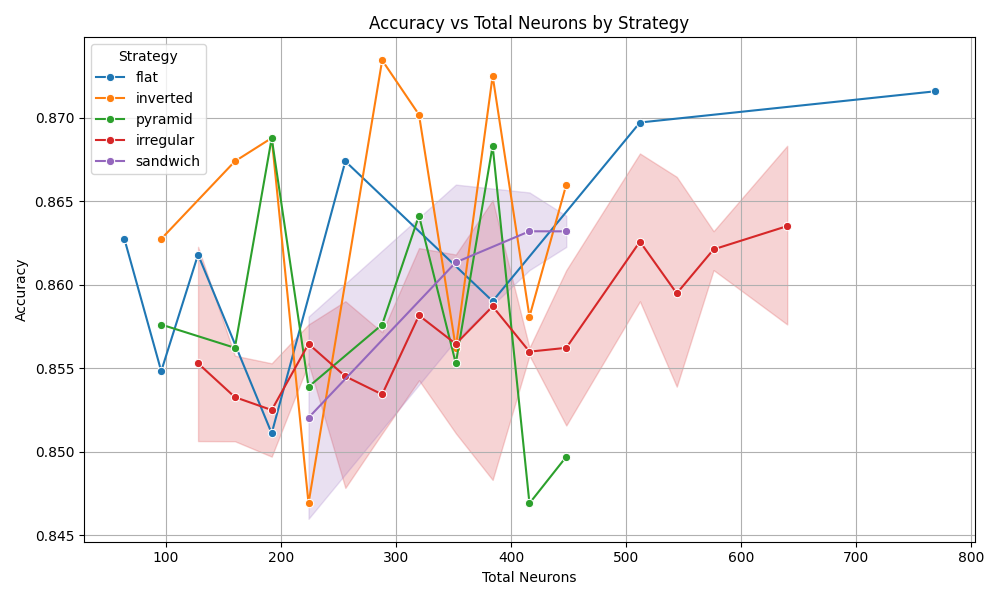
\includegraphics[width=0.9\textwidth]{/home/nikolis/Desktop/5o_etos/ai/predicting_alzheimers/screenshots/5.png}
    \label{fig:double}
\end{figure}

Οι καλύτερες αρχιτεκτονικές είναι οι inverted,pyramid και flat.Οι δύο πρώτες δίνουν καλύτερα αποτελέσματα μικρό/μεσαίο αριθμό νευρώνων ενώ η flat 
έχει έναν ποιο σταθερό ρυθμό που για κάθε τύπου αριθμό έχει καλές τιμές.H flat και η inverted επιτυγχάνουν accuracy μεγαλύτερο του 0,87.\\
Τέλος όπως φαίνεται και στον πίνακα οι 5 καλύτερες στρατηγικές έχουν πολύ καλές μέσες τιμές, δηλαδή αυξάνουν την αποδοτικότητα γενικά της εκπαίδευσης σε 
σχέση με 1 επίπεδο, ενώ οι χειρότερες δεν δίνουν κάποια βελτίωση.

\begin{table}[h!]
    \centering
    \caption{Best Configurations Based on Accuracy}
    \label{tab:top-architectures}
    \begin{tabular}{c c c c c c c}
    \hline
    \textbf{Architecture} & \textbf{Strategy} & \textbf{Num Layers} & \textbf{Run Epochs} & \textbf{Accuracy} & \textbf{MSE} & \textbf{Loss} \\
    \hline
    32,256       & inverted & 2 & 1048 & 0.873429 & 0.095236 & 0.396349 \\
    128,256      & inverted & 2 & 1043 & 0.872495 & 0.095589 & 0.397617 \\
    256,256,256  & flat     & 3 & 1102 & 0.871566 & 0.097962 & 0.448519 \\
    64,256       & inverted & 2 & 1057 & 0.870171 & 0.095272 & 0.395603 \\
    256,256      & flat     & 2 & 1049 & 0.869702 & 0.096572 & 0.399879 \\
    \hline
    \end{tabular}
    \end{table}

\begin{table}[h!]
    \centering
    \caption{Worst Configurations Based on Accuracy}
    \label{tab:worst-configs}
    \begin{tabular}{c c c c c c c c}
    \hline
     \textbf{Architecture} & \textbf{Strategy} & \textbf{Num Layers} & \textbf{Run Epochs} & \textbf{Accuracy} & \textbf{MSE} & \textbf{Loss} \\
    \hline
     256,64,64  & irregular & 3 & 1078 & 0.848305 & 0.111066 & 0.616754 \\
     128,64,64  & irregular & 3 & 1100 & 0.847828 & 0.112792 & 0.623555 \\
     32,64,128  & inverted  & 3 & 1100 & 0.846906 & 0.107798 & 0.559700 \\
     256,128,32 & pyramid   & 3 & 1100 & 0.846904 & 0.108825 & 0.587678 \\
     32,128,64  & sandwich  & 3 & 1100 & 0.845978 & 0.109213 & 0.585184 \\
    \hline
    \end{tabular}
    \end{table}


    \begin{figure}[H]
        \centering
        \includegraphics[width=0.9\textwidth]{/home/nikolis/Desktop/5o_etos/ai/predicting_alzheimers/screenshots_l1/best/Plot.png}
        \label{fig:double}
        \caption{Η [32,256] έχει το πιο ομαλό plot και παρουσιάζει το λιγότερο overfitting όπως φαίνεται. }
    \end{figure}  

    \begin{figure}[H]
        \centering
        \includegraphics[width=0.9\textwidth]{/home/nikolis/Desktop/5o_etos/ai/predicting_alzheimers/screenshots_l1/worst/Plot.png}
        \label{fig:double}
        \caption{Η [256,64,64] έχει την χειρότερη απόδοση και η απόσταση μεταξύ των losses αυξάνεται με μεγάλο ρυθμό. }
    \end{figure}  

Σημείωση:Οι υπόλοιπες φωτογραφίες των loss plots δεν συμπεριλαμβάνονται στην αναφορά για εξοικονόμηση χώρου(είναι 80 συνολικά), αλλά υπάρχουν στο github
και οι καλύτερες αρχιτεκτονικές είναι το ίδιο ομαλές με τη [32,256] , ενώ οι χειρότερες παρουσιάζουν το ίδιο πρόβλημα με τη [32,128,64].


\subsubsection{Αποδοτικότητα του αριθμού των κρυφών επιπέδων}

\begin{figure}[H]
    \centering
    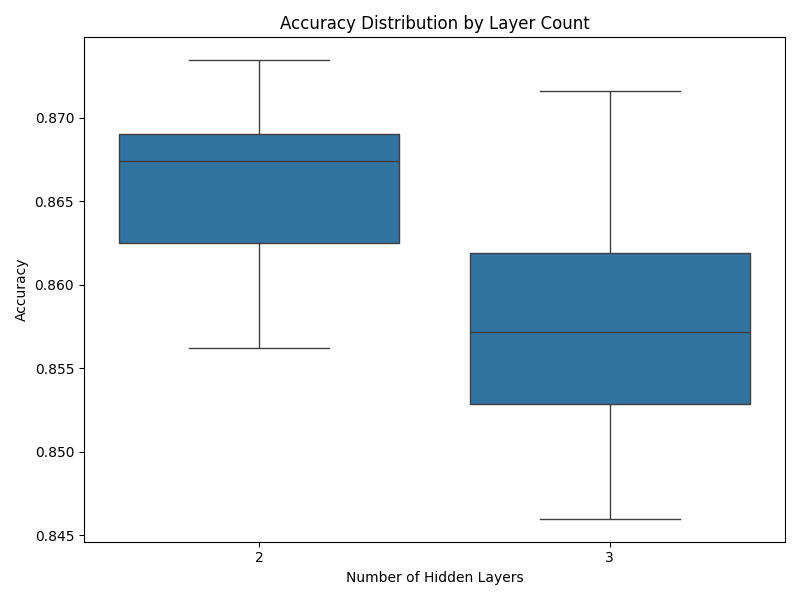
\includegraphics[width=0.9\textwidth]{/home/nikolis/Desktop/5o_etos/ai/predicting_alzheimers/screenshots/6.png}
    \label{fig:double}
\end{figure}

Για L1 καλύτερη απόδοση έχει ο μικρότερος αριθμός των επιπέδων(2), το οποίο είναι λογικό καθώς σε  ένα πιο απλό μοντέλο
ένα απλό tuning των weights είναι πιο αποδοτικό για την καταπολέμηση του overfitting.Σε ένα πιο πολύπλοκο δίκτυο όμως 
χρειάζεσαι μια πιο προσεκτική προσέγγιση(L2).


\subsubsection{Αριθμός epochs για σύγκλιση}


\begin{figure}[H]
    \centering
    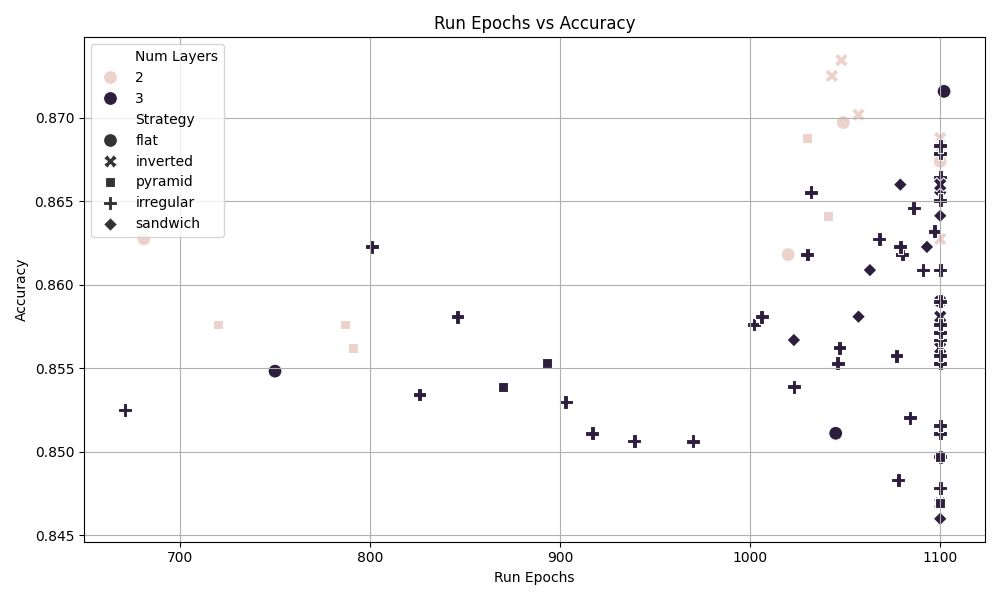
\includegraphics[width=0.9\textwidth]{/home/nikolis/Desktop/5o_etos/ai/predicting_alzheimers/screenshots/7.png}
    \label{fig:double}
\end{figure}

Χρειάζεται μεγαλύτερος αριθμός epochs για να συγκλίνει εκπαίδευση(400-500 παραπάνω) σχεδόν για όλους τους συνδυασμούς, το οποίο είναι
λογικό καθώς ο μεγαλύτερος αριθμός νευρώνων + επιπέδων + αργή συνάρτηση Regularization(όπως διαπιστώθηκε σε προηγούμενο ερώτημα) 
καθιστά πιο αργή(αλλά πιο ακριβή την εκπαίδευση).


\subsection{Δοκιμές με L2}

\subsubsection{Ακρίβεια-Αρχιτεκτονική-Αριθμός Νευρώνων}

\begin{figure}[H]
    \centering
    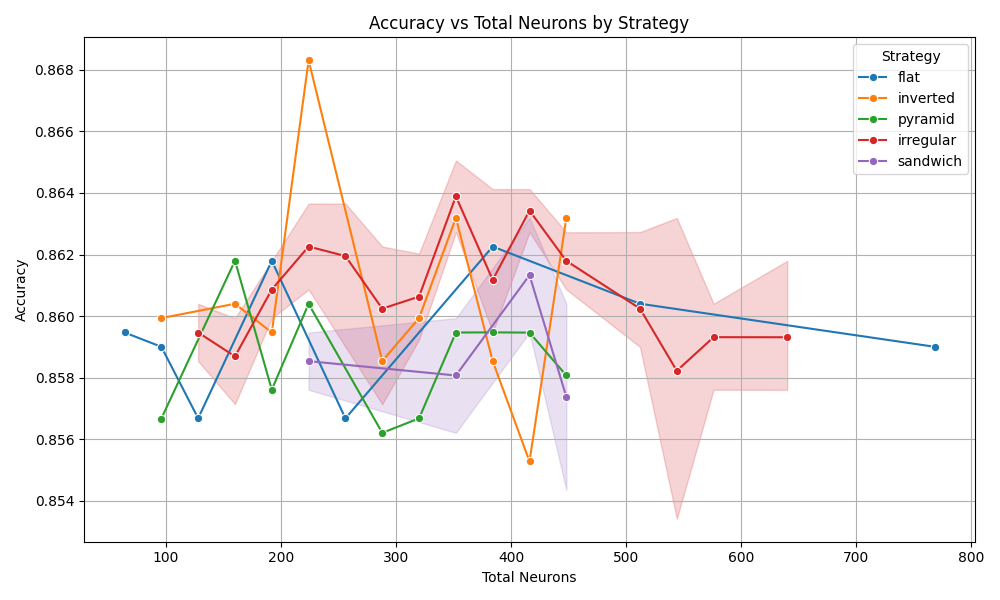
\includegraphics[width=0.9\textwidth]{/home/nikolis/Desktop/5o_etos/ai/predicting_alzheimers/screenshots/8.png}
    \label{fig:double}
\end{figure}

\begin{table}[h!]
    \centering
    \caption{Top 5 Best Architectures}
    \label{tab:best-architectures}
    \begin{tabular}{c c c c c c c}
    \hline
    \textbf{Architecture} & \textbf{Strategy} & \textbf{Num Layers} & \textbf{Run Epochs} & \textbf{Accuracy} & \textbf{MSE} & \textbf{Loss} \\
    \hline
    32,64,128   & inverted  & 3 & 721 & 0.868307 & 0.100675 & 0.446260 \\
    256,32,64   & irregular & 3 & 652 & 0.865052 & 0.099490 & 0.432573 \\
    256,32,128  & irregular & 3 & 670 & 0.864124 & 0.102504 & 0.438658 \\
    64,64,256   & irregular & 3 & 730 & 0.864122 & 0.100610 & 0.450053 \\
    128,32,64   & irregular & 3 & 665 & 0.863654 & 0.101460 & 0.433669 \\
    \hline
    \end{tabular}
    \end{table}
Παρόμοια αποτελέσματα με πριν με τη μόνη διαφορά η irregular αρχιτεκτονική(όχι κάποιο μοτίβο) έχει πάρει την θέση της πυραμίδας.Πάλι η inverted 
δίνει την καλύτερη μετρική η οποία είναι πάλι στην κλίμακα του 0,87.Οι καλύτερες αποδόσεις για όλες τις αρχιτεκτονικές είναι για μικρό/μεσαίο αριθμό νευρώνων.

\begin{figure}[H]
    \centering
    \includegraphics[width=0.9\textwidth]{/home/nikolis/Desktop/5o_etos/ai/predicting_alzheimers/screenshots/best/Plot.png}
    \label{fig:double}
    \caption{Η σύγκλιση είναι πιο γρήγορη σε σχέση με την L1 ,ίδιο ομαλή με μικρή διαφορά στην ακρίβεια}
\end{figure} 

Σημείωση: Οι χειρότερες περιπτώσεις δεν περιλαμβάνονται αλλά υπάρχουν και πάλι στο github, γιατί βγάζω το ίδιο συμπέρασμα με πριν.


\subsubsection{Αποδοτικότητα του αριθμού των κρυφών επιπέδων}

\begin{figure}[H]
    \centering
    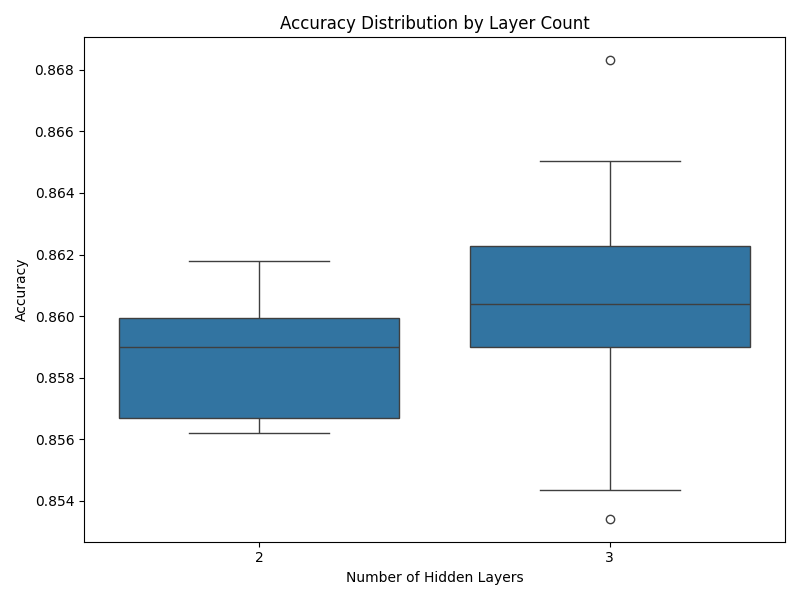
\includegraphics[width=0.9\textwidth]{/home/nikolis/Desktop/5o_etos/ai/predicting_alzheimers/screenshots/9.png}
    \label{fig:double}
\end{figure}

Όπως παρατηρήθηκε και πριν η L2 είναι καλύτερη για μεγαλύτερο αριθμό κρυφών επιπέδων.

\subsubsection{Αριθμός epochs για σύγκλιση}
\begin{figure}[H]
    \centering
    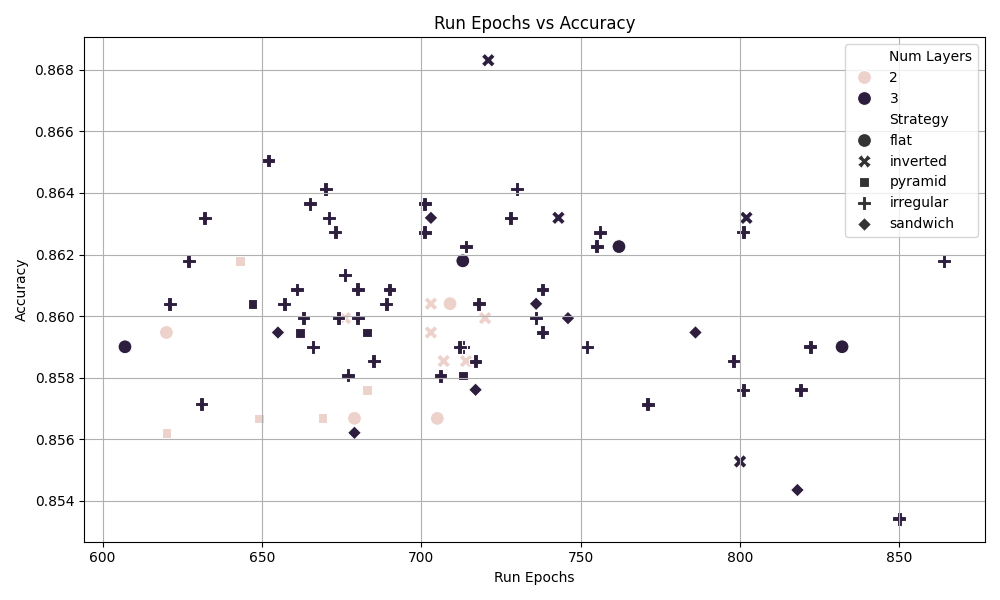
\includegraphics[width=0.9\textwidth]{/home/nikolis/Desktop/5o_etos/ai/predicting_alzheimers/screenshots/10.png}
    \label{fig:double}
\end{figure}

Οι περισσότερες προσπάθειες συγκλίνουν στα 650-750 epochs, περισσότερα από 1 μόνο επίπεδο αλλά καλύτερο ποσοστό ακρίβειας/epochs σύγκλισής από την L1. 

\subsection{Συμπέρασμα πειραμάτων πολλών επιπέδων}
Γενικά τα περισσότερα επίπεδα δίνουν μεγαλύτερη ακρίβεια από το 1 αλλά χρειάζονται περισσότερο χρόνο για να συγκλίνουν.Η αρχιτεκτονική εξαρτάται όπως είδαμε 
από το Regularization αλλά και στις 2 περιπτώσεις τα καλύτερα αποτελέσματα τα έδωσε η inverted αρχιτεκτονική για σχετικά μικρό αριθμό νευρώνων:
\begin{itemize}
    \item 32+64+128=224 για την L2
    \item 32+256=288 για την L1
\end{itemize}
Ο αριθμός των κρυφών επιπέδων εξαρτάται και πάλι απο το αν θα χρησιμοποιήσεις L1,L2 αλλά και οι 2 περιπτώσεις δίνουν πολύ καλές μέσες μετρικές.\\
Τέλος, οι πάρα πολλοί ή λίγοι  νευρώνες και η λάθος αρχιτεκτονική ενώ μπορεί να δίνουν καλύτερα αποτελέσματα από 1 κρυφό επίπεδο δεν αξιοποιούν την πλήρη δύναμη 
των κρυφών επιπέδων, λόγω των εξής προβλημάτων:
\begin{itemize}
    \item Uderfitting ή overfitting σε συνδυασμό με λάθος αρχιτεκτονική, κάθε επίπεδο δέν έχει το σωστό αριθμό νευρώνων για να μάθει τον τύπο των χαρακτηριστικών του και δεν υπάρχει σωστή διασύνδεση μεταξύ 
    επιπέδων, δηλάδή σωστός τρόπος και όγκος μεταφοράς πληροφορίας π.χ.(L1):
    \begin{table}[h!]
        \centering
        \label{tab:selected-architectures}
        \begin{tabular}{c c c c c c c c}
        \hline
         \textbf{Architecture} & \textbf{Strategy} & \textbf{Num Layers} & \textbf{Run Epochs} & \textbf{Accuracy} & \textbf{MSE} & \textbf{Loss} \\
        \hline
        256,128,32 & pyramid  & 3 & 1100 & 0.846904 & 0.108825 & 0.587678 \\
        256,64,64  & irregular & 3 & 1078 & 0.848305 & 0.111066 & 0.616754 \\
        \hline
        \end{tabular}
        \end{table}
    \item Η αρχικτεκτονική των δικτύων επηρεάζει τον τρόπο με τον όποιο συγκλίνει ο SGD π.χ. η sandwich αρχιτεκτονική και στις 2 περιπτώσεις είναι πολύ  κακή αρχιτεκτονική για πολλές τιμές.
\end{itemize}

\section{Συνολικά Συμπεράσματα}
 Συνοψίζοντας:
\begin{itemize}
    \item Για pre-processing η καλύτερη μέθοδος είναι η z-score
    \item Οι καλύτερες παράμετροί είναι οι : η=0.001,m=0.6,L1(r)=0.001
    \item Για περισσότερα του ενός κρυφού επιπέδου σε συνδυασμό με την Regularization function που χρησιμοποιείται, αυξάνεται η ακρίβεια, η εκπαίδευση παραμένει ομαλή 
    αλλά χρειάζεται περισσότερος χρόνος για την ολοκλήρωση της εκπαίδευσης.
\end{itemize}

\newpage
\section{Πράρτημα με πληροφορίες για τον κώδικα}
Το βασικό αρχείο είναι το alzheimers\_prediction.py.Χρησιμοποιείται parser για να μπορεί ο χρήστης δυναμικά να βάζει επιλογές για την εκπαίδευση.Πέρα απο το βασικό αρχείο 
υπάρχουν τα results.py και deep\_results.py για να βγάλω διάφορες μετρικές για το 1 και τα πολλά layers αντίστοιχα.\\
Τέλος υπάρχει το run.py/deep\_run.py που τρέχει όλες τις τιμές που ζητούνται και ο φάκελος screenshots που για τα plots.

\vspace{4em}
\textbf{Οι επιλογές με τις οποίες μπορεί να τρεχτεί το alzheimers\_prediction.py:}

\begin{description}
    \item[\texttt{--pre\_processing}] \textbf{Type:} \texttt{str}, \textbf{Default:} \texttt{"z-score"}\\
    Επιλογή της pre-processing μεθόδου, default:z-score.
  
    \item[\texttt{--optimizer}] \textbf{Type:} \texttt{str}, \textbf{Default:} \texttt{"adam"}\\
    Επιλογή Optimizer, default:adam
    \item[\texttt{--lr}] \textbf{Type:} \texttt{float}, \textbf{Default:} 0.001\\
    Επιλογή του η, default:0.001
  
    \item[\texttt{--momentum}] \textbf{Type:} \texttt{float}, \textbf{Default:} 0.0\\
    Επιλογή του m για τον SGD, default:0
  
    \item[\texttt{--epochs}] \textbf{Type:} \texttt{int}, \textbf{Default:} 50\\
    Τα epochs εκπαίδευσης.
  
    \item[\texttt{--num\_of\_layers}] \textbf{Type:} \texttt{str}, \textbf{Default:} \texttt{"two thirds"}\\
    Ο αριθμός των layers. Επιλογές: \texttt{I/2}, \texttt{2*I/3}, \texttt{I}, \texttt{2*I}.
  
    \item[\texttt{--loss\_func}] \textbf{Type:} \texttt{str}, \textbf{Default:} \texttt{"cross entropy"}\\
    Το loss function. Επιλογές: cross entropy, MSE.
  
    \item[\texttt{--hid\_layer\_func}] \textbf{Type:} \texttt{str}, \textbf{Default:} \texttt{"Relu"}\\
    Συνάρτηση ενεργοποίησης για τα κρυφά επίπεδα. Επιλογές: Relu, Tanh, Silu.
  
    \item[\texttt{--r}] \textbf{Type:} \texttt{float}, \textbf{Default:} None\\
    Το r, default:0.
  
    \item[\texttt{--all\_weights}] \textbf{Type:} \texttt{bool}, \textbf{Default:} False\\
    Τρέξιμο για όλες τις τιμές των βαρών χωρίς early stop.
  
    \item[\texttt{--test\_lr\_moment}] \textbf{Type:} \texttt{bool}, \textbf{Default:} False\\
    Παρόμοια για τα ζευγάρια η,m.
  
    \item[\texttt{--test\_reg}] \textbf{Type:} \texttt{bool}, \textbf{Default:} False\\
    Παρόμοια για τα r.
  
    \item[\texttt{--normal}] \textbf{Type:} \texttt{bool}, \textbf{Default:} True\\
    Κανονική εκπαίδευση με βάση τις παραμέτρους.
  
    \item[\texttt{--compare\_losses}] \textbf{Type:} \texttt{bool}, \textbf{Default:} False\\
    Δείχνει τα loss plots ξεχωριστά για κάθε fold και όχι το μέσο όρο τους.
  
    \item[\texttt{--more\_layers}] \textbf{Type:} \texttt{bool}, \textbf{Default:} False\\
    Χρήση περισσότεων layers.
  
    \item[\texttt{--use\_l2}] \textbf{Type:} \texttt{bool}, \textbf{Default:} False\\
    L2 regularization.
  
    \item[\texttt{--use\_l1}] \textbf{Type:} \texttt{bool}, \textbf{Default:} False\\
    L1 regularization.
  
    \item[\texttt{--hidden\_layers}] \textbf{Type:} \texttt{str}, \textbf{Default:} \texttt{""}\\
    Η αρχιτεκτονική του βαθύ δικτύου π.χ.: "32,256".
  \end{description}

  \textbf{Παράδειγμα χρήσης:}
  \begin{minted}[frame=single, linenos, fontsize=\footnotesize]{bash}
python3 alzheimers_prediction.py --optimizer SGD --epochs 600 --num_of_layers double \
--lr 0.001 --momentum 0.6 --use_l1 True --r 0.001 
    \end{minted}
  
Σημείωση:Τα αποτελέσματα αποθηκεύνται στην mongoDB, προσοχή όταν τρέχετε το py αρχείο.\\
Το github θα γίνει προσβάσιμο ακριβώς μετά την λήξη της προθεσμίας για λόγους αντιγραφής.


\end{document}
